\documentclass[UTF8]{ctexart}
\usepackage{amsmath}
\usepackage{amssymb}
\usepackage{graphicx}
\author{张志博 2017211416}
\title{机器学习-第2次作业}
\begin{document}
\maketitle

\section{《统计学习方法》}习题7.1、7.2
\subsection{习题7.1}
\paragraph{比较感知机的对偶形式与线性可分支持向量机的对偶形式。}
\subsubsection{对偶形式}
\paragraph{对偶形式的基本思想是,将$w$和$b$表示为实例$x_i$和标记$y_i$的线性组合的形式,通过求解其系数而求得$w$和$b$,对误分类点$(x_i,y_i)$通过}
\begin{align*}
    \begin{cases}
        w\leftarrow w+\mu y_{i}x_{i} \\
        b\leftarrow b+\mu y_{i}
    \end{cases}
\end{align*}
\paragraph{逐步修改$w,b$,设修改$n$次,则$w,b$关于$(x_i,y_i)$的增量分别是$\alpha_{i}y_{i}x_{i}$和$\alpha_{i}y_{i}$,这里$\alpha_{i}=n_{i}\mu$。最后学习到的$w,b$可以分别表示为}
\begin{align*}
    \begin{cases}
        w=\sum\limits_{i=1}^{N}\alpha_{i}y_{i}x_{i} \\
        b=\sum\limits_{i=1}^{N}\alpha_{i}y_{i}
    \end{cases}
\end{align*}

\subsubsection{感知机学习算法的对偶形式}
\paragraph{输入:线性可分的数据集$T=\{(x_1,y_1),(x_2,y_2),\dots(x_N,y_N))\}$,其中$x_i\in R^n$,$y_i\in {-1,+1}$,$i=1,2,\dots,N$;学习率$\mu(0<\mu\le 1)$}
\paragraph{输出:$\alpha$,$b$;感知机模型$f(x)=sign(\sum\limits_{j=1}^{N} \alpha_{j}y_{j}x_{j}x+b)$。其中$\alpha=(\alpha_1,\alpha_2,\dots,\alpha_N)^T$}
\paragraph{(1)}
\begin{align*}
    \begin{cases}
        \alpha\leftarrow 0 \\
        b\leftarrow 0
    \end{cases}
\end{align*}
\paragraph{(2) 在训练集中选取数据$(x_i,y_i)$}
\paragraph{(3) 如果$(\sum\limits_{j=1}^{N} \alpha_{j}x_{j}y_{j}x_{i}+b)\le 0$}
\begin{align*}
    \begin{cases}
        \alpha_{i}\leftarrow\alpha_{i}+\mu \\
        b\leftarrow b+\mu y_{i}
    \end{cases}
\end{align*}
\paragraph{(4) 转至(2)直至没有误分类数据}
\paragraph{$w,b$实质是将其表示为$x_i,y_i$的线性组合形式:}
\begin{align*}
    \begin{cases}
        w=\sum\limits_{i=1}^{N}\alpha_i^*j_ix_i \\
        b=\sum\limits_{i=1}^{N}\alpha_i^*j_i
    \end{cases}
\end{align*}

\subsubsection{支持向量机学习算法的对偶形式}
\paragraph{原始问题的对偶问题是}
\begin{align*}
    \begin{cases}
        \min\limits_{\alpha}\frac{1}{2}\sum\limits_{i=1}^{N}\sum\limits_{j=1}^{N}\alpha^i\alpha^j y^i y^j x_i x_j-\sum\limits_{i=1}^{N}\alpha_i\\
        s.t. \ \sum\limits_{i=1}^{N}\alpha_i y_i=0 \\
        0\le\alpha_i\le C,\ i=1,2,\dots,N
    \end{cases}
\end{align*}
\paragraph{求解对偶问题后得到的$w,b$实质是将其表示为$x_i,y_i$的线性组合形式:}
\begin{align*}
    \begin{cases}
        w^*=\sum\limits_{i=1}^{N}\alpha_i^*j_ix_i \\
        b^*=y_j-\sum\limits_{i=1}^{N}\alpha_i^*x_ij_i
    \end{cases}
\end{align*}

\subsection{习题7.2}
\paragraph{试求最大间隔分离超平面和分类决策函数,并在图上画出分离超平面、间隔边界及支持向量。}
\paragraph{使用了Python的库numpy、matplotlib.pyplot、sklearn.svm,采用线性核的SVM,惩罚系数C=10(因为数据集过小,所以采用了很高的惩罚系数,这样结果和手动计算得到的系数更加接近),计算后得到结果,最大间隔分离超平面:$-x+2y-2=0$,分类决策函数为$f(x)=sign(-x+2y-2=0)$}
\begin{figure}[htp]
    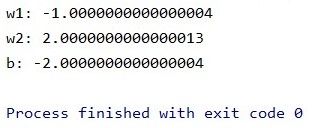
\includegraphics{Screenshot.jpg}
\end{figure}
\paragraph{分离超平面、间隔边界及支持向量如上图}
\begin{figure}[htp]
    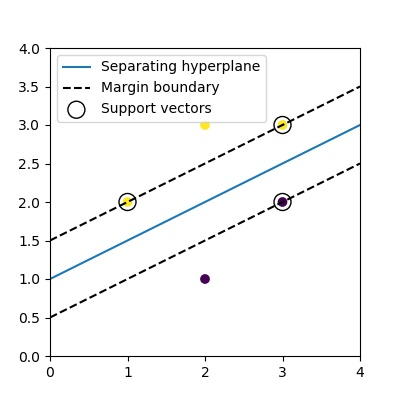
\includegraphics[width=9cm, height=9cm]{fig.jpg}
\end{figure}
\paragraph{}


\section{《机器学习》}习题6.3
\subsection{习题6.3}
\paragraph{选择两个UCI数据集,分别用线性核和高斯核训练一个SVM,与C4.5决策树进行实验比较}
\paragraph{训练集、测试集的划分使用了sklearn.model\_selection.train\_test\_split,具体参数如下图,训练集和测试集比例为7:3,让random\_state=1使几次训练集和测试集的划分一致,减少无关变量。}
\paragraph{使用了Python的库sklearn,计算后得到结果}
\paragraph{}
\begin{figure}[htp]
    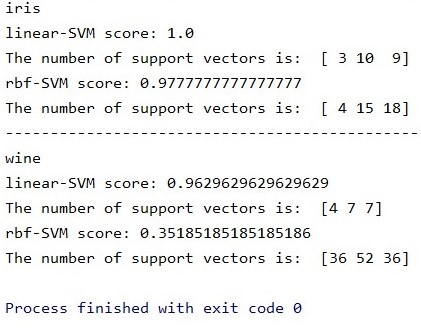
\includegraphics{svm.jpg}
\end{figure}
\paragraph{对于数据集iris,用线性核训练的SVM,总共有22个支持向量,在测试集上的准确率是100\%,由此可见,iris数据集是线性可分的;
用高斯核训练的SVM,总共有37个支持向量,在测试集上的准确率是97.8\%,效果不如线性核;}
\paragraph{对于数据集wine,用线性核训练的SVM,总共有18个支持向量,在测试集上的准确率是96.3\%;
用高斯核训练的SVM,总共有124个支持向量,然而数据大小才只有178,在测试集上的准确率只有35.2\%,可能是由于特征过多,也可能是因为使用默认参数,导致发生了过拟合。}
\paragraph{}
\begin{figure}[htp]
    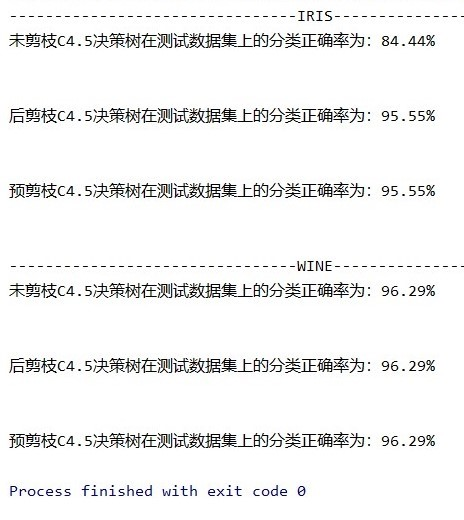
\includegraphics{c45.jpg}
\end{figure}
\paragraph{对于数据集iris,用后剪枝的C4.5决策树在测试集上的准确率是95.6\%,低于SVM方法;
对于数据集wine,用C4.5决策树在测试集上的准确率是96.3\%,低于线性核训练的SVM,高于高斯核训练的SVM。}

\end{document}

